% simulation.tex
The purpose of the simulations is to allow for better understanding of
the behavior of platforms interconnecting structured overlay networks
through the Synapse approach. We focus on the key metrics
traditionally considered in distributed information retrieval process,
such as exhaustiveness (the extent of existing objects effectively
retrieved by the protocol), latency (number of hops required to reach
the requested object) and the amount of communications produced
(number of messages generated for one request). We want to highlight
the behavior of these metrics while varying the topology (the number
of synapses and their connectivity, TTL, the number of intra-overlays
...).

%\subsection{Settings}
%
\noindent{\bf Settings.}
%
Our simulations have been conducted using Python scripts, and using
the \emph{white box} protocol, capturing the essence of the Synapse
approach. The topology of the overlay simulated is a set of Chord
networks interconnected by some synapses.  Information is a set of
{\tt (key,value)} pairs. Each pair is unique and exists once and only
once in the network. We study the unstructured interconnection of
structured networks. We used discrete-time simulation: queries are
launched on the first discrete time step, initiating a set of messages
in the network, and each message sent at the current step will be
received by its destination (next routing hop) at the next hop.

%\subsection{Synapses}
%
\noindent{\bf Synapses.}
%
Our first set of simulations has the intent of studying how the
previously mentioned metrics vary while we add synapses or increase
the degree of existing ones (the number of intra-overlays a co-located
node belongs to). The number of nodes was fixed to $10000$, uniformly
distributed amongst $20$ overlays (approximately $500$ nodes within
each Chord). Queries are always triggered by one random node, the key
sought by a query is also picked uniformly at random among the set of
keys stored by the network. A query is said to be \emph{satisfied} if
the pair corresponding to the key has been successfully retrieved.

We first studied search latency, \ie\ the number of hops to obtain the
first successful response.
% (if the keys searched were stored on several overlays, the latency
% would correspond to the first response received).
As illustrated in Figure~\ref{fig:3D-hops}, one first point to notice
is that the number of hops remains logarithmic when changing a Chord
network into a Synapse network (the number of nodes is $10000$, the
latency never exceeds 14). Other experiments conducted by increasing
the number of nodes confirm this. More precisely,
Figure~\ref{fig:3D-hops} (left) highlights the following behavior:
$(i)$ when the network contains only a few synapses, the latency first
increases with the degree of synapses: only a few \emph{close} keys
are retrieved (keys available in the network of the node that
initiated the query); $(ii)$ then, when both parameters (the
connectivity and the number of synapses) have reached a certain
threshold, the searches can touch more synapses, and the whole network
becomes progressively visible, multiple parallel searches become more
and more frequent and distant nodes (and keys) are reached faster. As
we can see, increasing the number of synapses decreases the latency of
only a small constant factor. In other words, synapse topologies does
not need a lot of synapses to be efficient. This result fits with
random graphs behavior: when the number of neighbors in the graph
reaches a (small) threshold, the probability for the graph to be
connected tends towards $1$.
% 
\begin{figure}[!t]
\up{4}
        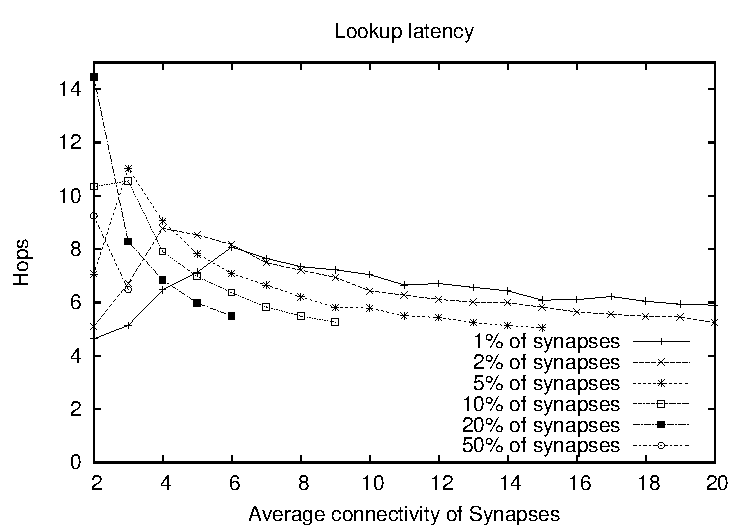
\includegraphics[width=0.5\linewidth]{fig/3D-hops.pdf}
        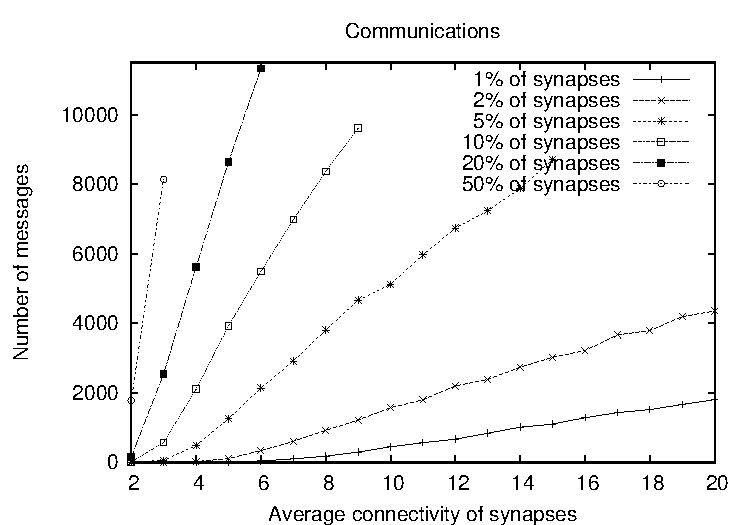
\includegraphics[width=0.5\linewidth]{fig/3D-msgs.pdf}
\up{4}
        \caption{Latency and communications in Synapse\label{fig:3D-hops}}
%\up{2}
\end{figure}
%
Obviously, multiple searches in parallel lead to an increased number
of messages. As illustrated in Figure~\ref{fig:3D-hops} (right), this
number increases proportionally with the connectivity and the number
of synapses. 
% A good-deal strategy in synapses can leverage this inter-network
% overhead.

% Moreover, the number of total communications tends to be linear in
% the number of nodes, which can obviously become a serious problem,
% as pointed out in unstructured networks.
%
% \begin{figure}
%   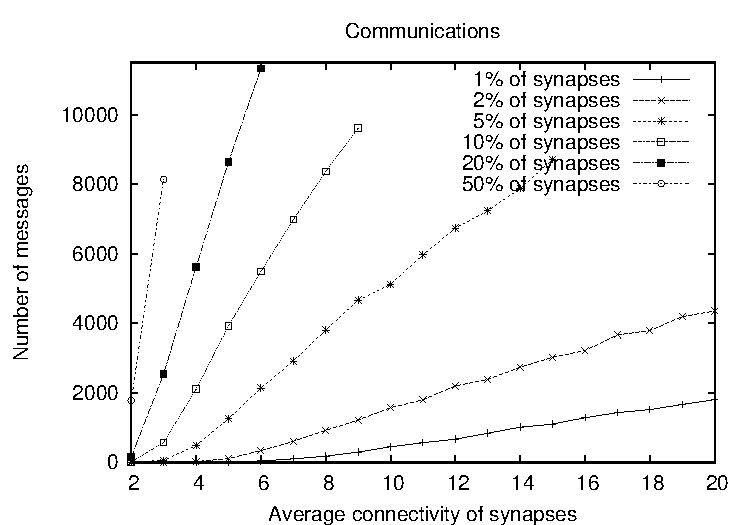
\includegraphics[width=0.5\linewidth]{fig/3D-msgs.pdf}
%   \caption{Synapses and communicationss\label{fig:3D-msgs}}
% \end{figure}

%%% TTL simulations

%\subsection{Time-To-Live}
%
\noindent{\bf Time-To-Live.}
As we pointed out, the number of messages can become high when the
number of synapses increases. To limit this impact, we introduced a
Time-to-Live (TTL) to reduce the overhead while keeping an acceptable
level of exhaustiveness.  We launched a second set of experiments in
order to study the impact of the TTL on the search queries. This TTL
is simply decreased every time the query traverses a node. 

The purpose is here is to preserve significant exhaustiveness, while
reducing the amount of communications undergone by the
inter-overlay. We made the number of overlays vary, to experiment the
impact of the \emph{granularity} of the network.  In other words, a
Synapse network made of few large structured intra-overlays could be
called \emph{strongly structured}, while another network with many
smaller structured intra-overlays could be called \emph{weakly
  structured}. The number of nodes was still set to $10000$, and every
node is a synapse belonging to $2$ overlays chosen uniformly at
random.


\begin{figure}[!t]
  \up{4}
  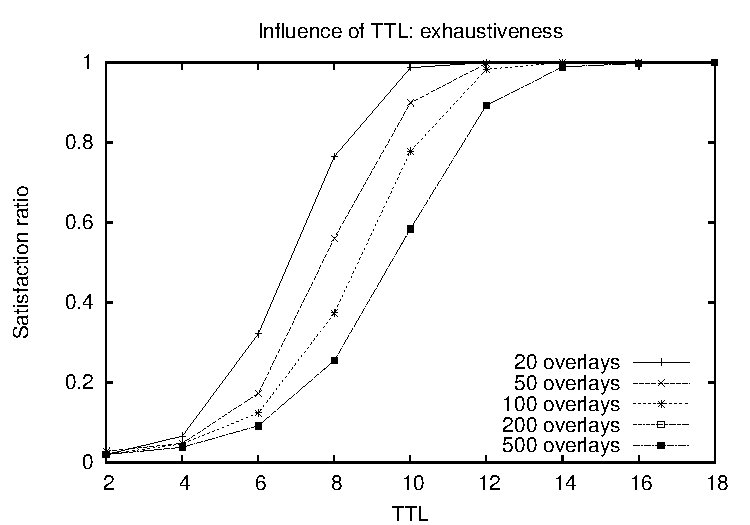
\includegraphics[width=0.5\linewidth]{fig/TTL-sat.pdf}
  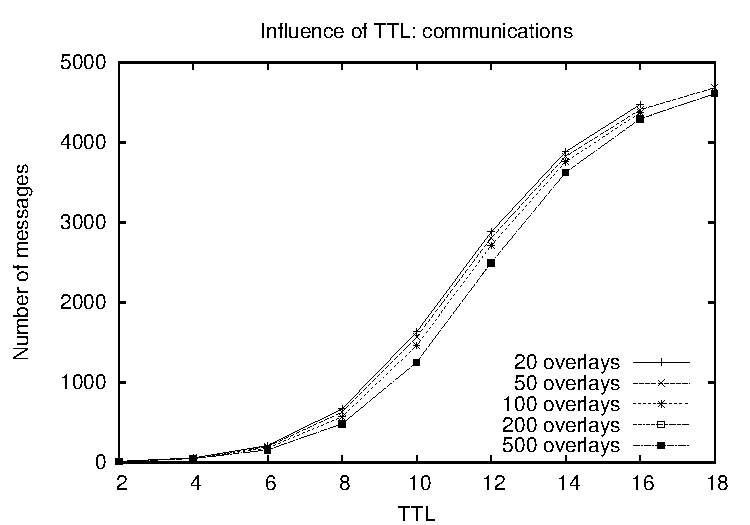
\includegraphics[width=0.5\linewidth]{fig/TTL-msgs.pdf}
  \up{4}
  \caption{TTL \vs\ exhaustiveness and communications\label{fig:TTL-sat}}
  \up{4}
\end{figure}
% 
% \begin{figure}
%   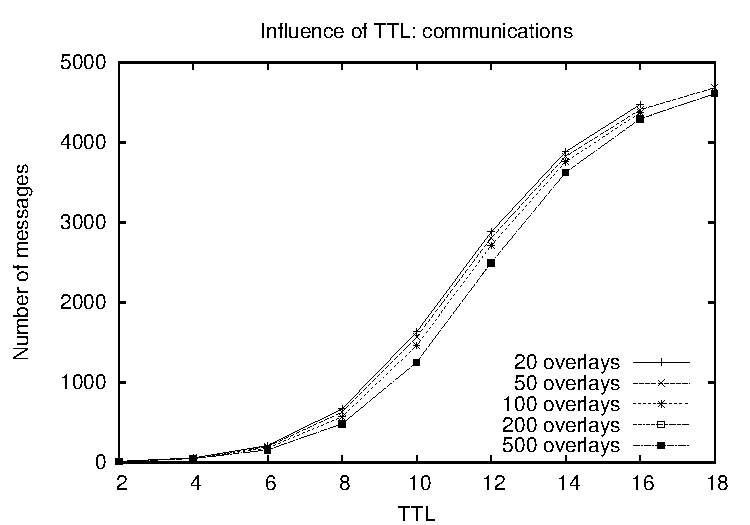
\includegraphics[width=0.45\linewidth]{fig/TTL-msgs.pdf}
%   \caption{TTL and communications\label{fig:TTL-msgs}}
% \end{figure}
%  
Figure~\ref{fig:TTL-sat} (left) confirms that a low synapse degree
($2$) is enough to achieve quasi-exhaustiveness. Another interesting
result is that TTL can be bounded without any impact on the
exhaustiveness ($10$ or $12$ is enough even when the number of
overlays interconnected is $500$), while, as highlighted by
Figure~\ref{fig:TTL-sat} (right), drastically reducing the amount of
communications experienced, with the number of messages being almost
divided by $2$. To sum up, Synapse architectures can use TTL, leading
to a significant exhaustiveness while drastically reducing the
expected overhead.
%
Finally, still see Figure~\ref{fig:TTL-sat}, the \emph{granularity}
(defined above) does not significantly influence exhaustiveness and
communications when the number and connectivity of the synapses are
fixed.

%\subsection{Connectivity and Peers' churn}
%
\noindent{\bf Connectivity and Peers' churn}
%
Figure~\ref{fig:3D-sat} (left) shows the evolution of the
exhaustiveness while increasing the average number of overlays a
synapse belongs to. We repeated the experiment for different ratios of
synapses (in percentage of the total number of nodes). The
exhaustiveness is improved by increasing both factors. We obtain more
than 80\% of satisfaction with only 5\% of nodes belonging to 10
floors, and other nodes belonging to only one intra-overlay. When each
node belongs to $2$ overlays, the exhaustiveness is also almost
guaranteed.

\begin{figure}[!t]
  \up{4}
  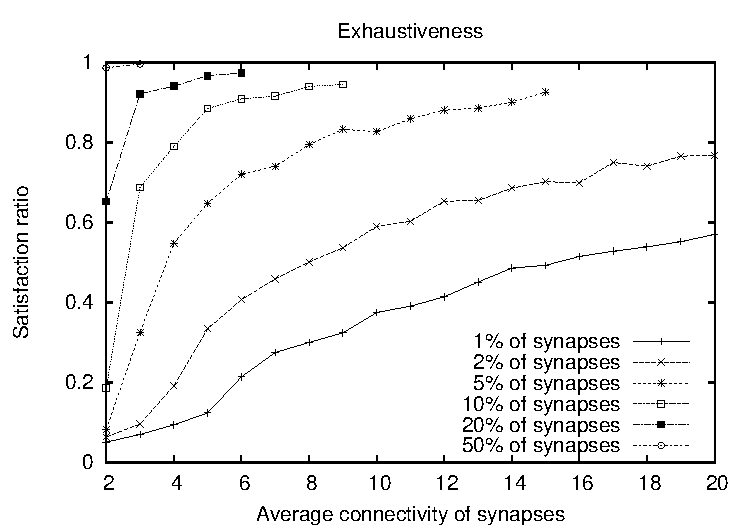
\includegraphics[width=0.5\linewidth]{fig/3D-sat.pdf}
  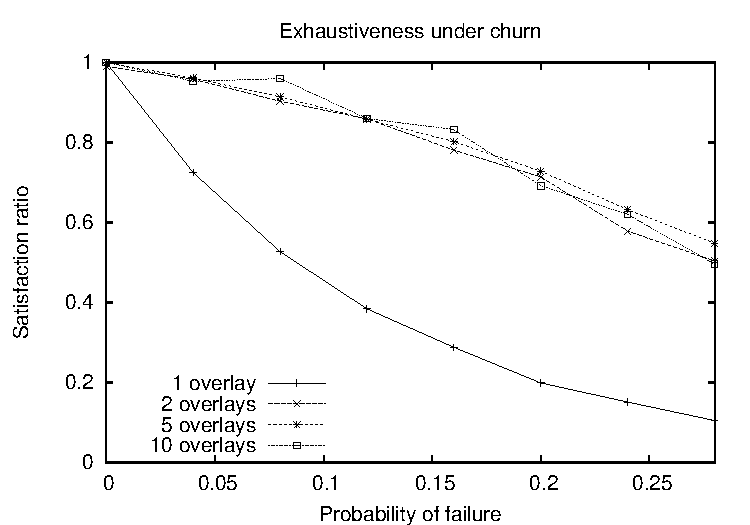
\includegraphics[width=0.5\linewidth]{fig/churn-sat.pdf}
  \up{4}
  \caption{Exhaustiveness \vs\ synapses and churn\label{fig:3D-sat}}
  \up{4}
\end{figure}
%
Since networks are intended to be deployed in a dynamic settings (nodes
joining and leaving the network without giving notice), we conducted a
final set of simulations to see the tolerance of Synapse compared to a
single Chord overlay network. In other words, the question is
\emph{Does an interconnection of small Chords better tolerate
  transient failures than one large unique Chord?} In this experiment,
at each step, a subset of nodes is declared unreachable (simulating
the churn), making message routing fail. As we can see on
Figure~\ref{fig:3D-sat} (right), improvement on the number of
satisfied requests can be obtained through a Synapse network: when the
probability of failure/disconnection of a node increases, the global
availability of the network is far less reduced with Synapse than with
Chord. This shows that such synapse architectures are more robust and
thus good candidates for information retrieval on dynamic platforms.
 